%!TEX root = main.tex

\section{Design rationale}

\label{sec:rationale}

% When we initially think about the transport control mechanism in new network architecture, the first question is who dominant and should be responsible for the congestion control? In TCP/IP, as its push principle, it is the senders who deal with the network congestion by changing the packet sending window. Under the pull nature of NDN, it is obviously that the receivers should be responsible for the network congestion. The one-Interest one-Data principle makes it possible to control the network traffic through the control of Interest sending rate. Such control congestion is called receiver-driven transport mechanism\cite{Contug}. Our design also follows the receiver-driven principle.

% If several flows share one link, it is ideal that the link bandwidth is ultimately used and at the same time fairly shared by all the flows. ECN information reflects the network resource situation such as that the available bandwidth and flow number of the path. By the ECN information, receivers can adjust its Interest sending rate to ultimately use the bandwidth and achieve fairness. So our first design goal is to use the ECN information to control the receiver's Interest sending rate.

% By controlling the receiver's Interest sending rate, we can perhaps ultimately use the link bandwidth and avoid congestion. But if all the flows choose a path that goes through the same bottleneck, even we can ultimately use the link bandwidth, the flow complete time can be low, because too many flows share the same bottleneck. So if there are several paths available for the flows, how can we choose different paths for different flows that minimum all the flows' complete time? Our second design goal is to design a smart forwarding mechanism that minimum flow complete time.

% In TCP/IP, the route path is single path, and the forwarding process is strictly follows the route path. Choosing path adaptively is very difficult. However, in NDN, the adaptive forwarding makes it possible. Take the mesh network topology in Fig. \ref{fig-topology}. as example. A flow goes through router5. The flow has two available paths to get the data from provider. Router5 can easily measure the congestion condition at the link1 (between router5-7) and link2 (between router5-8). If the router senses that link1 is much more congested than link2 then the router can adaptively forward the flow to link2. By such adaptive forwarding, the network resource can be effectively used and reduce the flow complete time.

% But such just one hop measure way is very limited. Take the same situation as example. The true bottleneck happens on link3 (between router10-13). But the router5 can measure just one hop situation, it cannot sense the true bottleneck is on the link3, so it will still forward the interest to link2. The wrong forwarding decision will add more burdens to link3, and reduce the flow complete time of all the flows.

% The SDN-style controller can get the whole network information. We will introduce the SDN's network-wide information to overcome the ��limited information�� problem. By the network-view information, the Interest can be forwarded to the best path. The whole network bandwidth utilization and total flow complete time can be improved.

When we to design transport control mechanism for a new network architecture, the first question is which entity should be responsible for the congestion control. In TCP/IP, as its push principle, it is the sender who deals with network congestion by adjusting the packet sending window. Under the pull nature of NDN, it is obvious that receivers should be responsible for the network congestion. The one-to-one mapping of Interest-Data makes it possible to control the network traffic through the control of Interest sending rate. Such control congestion is called receiver-driven transport mechanism\cite{Contug}. Our design also follows the receiver-driven principle.

If multiple flows are transmitted through one link, it is ideal that the link bandwidth is fully utilized and at the same time fairly shared by all the flows. ECN information reflects the network resource situation such as the available bandwidth and the number of flows on the path. According to the ECN information, receiver adjusts its Interest sending rate to fully use the bandwidth and achieve fairness. So to fully use link bandwidth we first use the ECN information to control the receiver's Interest sending rate.

By controlling receivers' Interest sending rate, we can perhaps fully use the link bandwidth and avoid congestion. But if all the flows choose a path that goes through the same bottleneck, even we can fully use the link bandwidth and achieve fairness, the flow complete time can be very low, because too many flows share the same bottleneck. So if there are several paths available for the flows, how can we allocate the multiple paths to each flow to minimize the total flow complete time?

In TCP/IP, only a single path is available for each source destination pair, and the forwarding process strictly follows the single path, thus adaptively selecting alternative path is very difficult. However, in NDN, the adaptive forwarding makes it possible. Taking the mesh network topology in Fig. \ref{mesh-topology} for example, a flow goes through $R5$. The flow has two available paths to get the data from provider. Router $R5$ can easily measure the congestion condition at the link1 (between router $R5$ and $R7$) and link2 (between router $R5$ and $R8$). If the router senses that link1 is much more congested than link2 then the router can adaptively forward the flow to link2. By such adaptive forwarding, the network resource can be effectively used and the flow complete time will be reduced.

\begin{figure}[t]
	\centering
	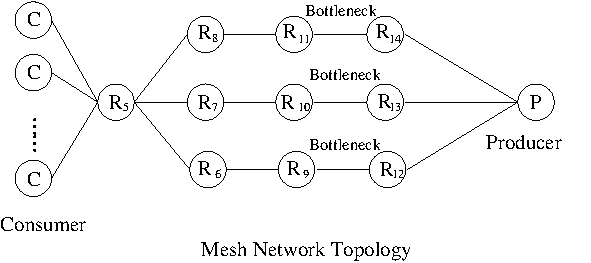
\includegraphics[width=2.5in]{mesh-topology.pdf}
	\caption{A mesh topology}
	\label{mesh-topology}
\end{figure}

However, such a one-hop measurement is very limited. Taking the same situation for example, the true bottleneck happens on link3 (between router $R10$ and $R13$). But the router $R5$ can measure just one hop situation, it cannot sense the true bottleneck is on the link3, so it will still forward the Interest to link2. The wrong forwarding decision will put more burdens to link3, and increase the flow complete time of all the flows.

The SDN-style controller can get the whole network information. We will introduce the SDN's network-wide information to overcome the ``limited information'' problem. By the network-view information, the Interest can be forwarded to the best path. The whole network bandwidth utilization will be improved and total flow complete time can be reduced. So to improve the whole network bandwidth utilization and minimize total flow complete time, we further use SDN's network-wide information to design smart forwarding mechanism.
